\section{Exemple d'implémentation d'un post-traitement dans \ansys}

Dans ce chapitre, nous présentons un manière d'implémenter la méthode «Reissner local» mentionnée aux paragraphes~\ref{Sec-PT} et~\ref{Sec-interf}.
Il s'agit de calculer les contraintes à l'interface entre deux matériaux en utilisant la fonctionnelle mixte d'Hellinger-Reissner\index[aut]{Reissner (Max Erich, dit Eric), 1913-1996, Américain}\index[aut]{Hellinger (Ernst David), 1883-1950, Allemand}\index{fonctionnelle!d'Hellinger-Reissner}\index{fonctionnelle!mixte}
donnée à l'équation (\ref{Eq-HR2}).

Le but est de montrer que même sur un maillage grossier, il est possible de correctement estimer les contraintes aux interfaces, pour peu que l'on dispose d'une méthode appropriée. Nous espérons qu'au passage, nous démontrerons également qu'il est assez simple d'implémenter des fonctions dans un code existant.


\medskip
\subsection{Macro dans \ansys}

Si un code ne dispose pas de la méthode que l'on souhaite utiliser, il est toujours possible de retraiter les résultats... toutefois, selon les codes, il est plus ou moins aisé d'implémenter des fonctions dans ledit code.

\medskip
\ansys est souvent qualifié de «code industriel», ce qui pourrait laisser supposer qu'il n'a pas la même capacité à résoudre les problèmes que des codes dits «de recherche» ou «spécialisés». Or il n'en est rien (même si en toute rigueur, il y a une quinzaine d'années il était plus faible que d'autres sur les non linéarités, ce qui n'est plus vrai depuis longtemps).

C'est vrai que disposant d'une interface utilisateur remarquable (comparée à celle de nombreux autres codes), il est possible de ne réaliser les calculs que via cette interface, i.e. sans passer par un fichier batch... ce que ne font de toutes façons pas les gens sérieux (donc cet argument ne tient pas).

Le qualificatif d'industriel peut également laisser penser que le logiciel est plus fermé que d'autres, mais ce n'est que partiellement le cas, en tous les cas on peut y remédier facilement, et c'est pourquoi nous allons présenter l'implémentation d'une macro dans ce code.

\medskip
Pour implémenter une nouvelle fonction dans \ansys, plusieurs méthodes s'offrent à nous. Nous citerons:
\begin{itemize}
  \item écrire le bout de programme et recompiler le noyau: c'est faisable en théorie, mais personnellement je n'ai jamais réussi...
  \item partir des fichiers de résultats binaires pour les retravailler: c'est également théoriquement faisable, mais 	il faut décortiquer les formats d'écriture desdits fichiers, les relire, réécrire dans le même format... et c'est donc beaucoup de travail (purement informatique);
  \item programmer la fonction directement sous \ansys (\ansys possède un langage assez riche et puissant);
  \item ou alors, et c'est la voie que nous allons montrer, utiliser \ansys en «coopération» avec un petit programme extérieur.
\end{itemize}

\medskip
La structure de la macro \ansys que nous proposons (et qui peut être également incluse dans les menus d'\ansys, mais nous n'entrons pas dans ce niveau de détail d'interfaçage) est très simple:
\begin{itemize}
  \item on récupère les données dont nous avons besoin et on les stocke dans des fichiers externes (simples);
  \item on lance un programme externe (dont la structure sera exposée plus bas);
  \item on réintègre les résultats dans \ansys.
\end{itemize}
On peut alors se servir de toutes les fonctions de visualisation disponibles dans \ansys avec les résultats modifiés...

\color{gris}\scriptsize
\begin{multicols}{2}
%\begin{verbatim}
\begin{Verbatim}[numbers=left,numbersep=3pt]
/nop
! Vincent MANET
! ENSM.SE, 1998
!
nall
!
! Parametres
*get,Nnoeuds,node,,count
*get,Nmater,mat,,count
*get,Nelem,elem,,count
*cfopen,temp,par
*vwrite,Nnoeuds
(E13.7,' ')
*vwrite,Nelem
(E13.7,' ')
*vwrite,Nmater
(E13.7,' ')
*cfclose
!
! Materiaux
*cfopen,temp,mat
*dim,Mater,,Nmater,3
*do,I,1,Nmater
  *get,Mater(I,1),Ex,I
  *get,Mater(I,2),Ey,I
  *get,Mater(I,3),Nuxy,I
*enddo
*vwrite,Mater(1,1),Mater(1,2),Mater(1,3)
(3(E13.7,' '))
*cfclose
!
! Noeuds
*dim,CoordX,,Nnoeuds
*dim,CoordY,,Nnoeuds
*dim,CoordZ,,Nnoeuds
*vget,CoordX(1),node,,loc,x
*vget,CoordY(1),node,,loc,y
*cfopen,temp,coo
*vwrite,CoordX(1),CoordY(1)
(2(E13.7,' '))
*cfclose
!
! Elements + numero du materiau
*dim,E1,,Nelem,9
*vget,E1(1,1),elem,1,node,1
*vget,E1(1,2),elem,1,node,2
*vget,E1(1,3),elem,1,node,3
*vget,E1(1,4),elem,1,node,4
*vget,E1(1,5),elem,1,node,5
*vget,E1(1,6),elem,1,node,6
*vget,E1(1,7),elem,1,node,7
*vget,E1(1,8),elem,1,node,8
*vget,E1(1,9),elem,1,attr,mat
*cfopen,temp,elt
*vwrite,E1(1,1),E1(1,2),E1(1,3),E1(1,4),E1(1,5),E1(1,6),
        E1(1,7),E1(1,8),E1(1,9)
(9(E13.7,' '))
*cfclose
!
! Resultats
*vget,CoordX(1),node,1,U,x
*vget,CoordY(1),node,1,U,y
*cfopen,temp,res
*vwrite,CoordX(1),CoordY(1)
(2(E13.7,' '))
*cfclose
!
! Contraintes
*vget,CoordX(1),node,1,S,x
*vget,CoordY(1),node,1,S,y
*vget,CoordZ(1),node,1,S,xy
*cfopen,temp,str
*vwrite,CoordX(1),CoordY(1),CoordZ(1)
(3(E13.7,' '))
*cfclose
!
! run locreiss.exe
/sys,'locreiss.exe'
!
! Effacer les fichiers
! generes par ANSYS:
!   - temp.par: parametres
!   - temp.coo: coordonnees nodales
!   - temp.elt: incidences
!   - temp.mat: proprietes materielles
!   - temp.res: deplacements nodaux
!   - temp.str: contraintes nodales
! generes par locreiss.exe:
!   - temp.dum
!   - temp.tmp
! Il reste les fichiers
!   - temp.sij: contraintes nodales modifiees
!
!/sys,'rm ./temp.par'
!/sys,'rm ./temp.coo'
!/sys,'rm temp.elt'
!/sys,'rm temp.mat'
!/sys,'rm temp.res'
!/sys,'rm temp.str'
!/sys,'rm temp.dum'
!/sys,'rm temp.tmp'
!
! lire les valeurs dans temp.sij
! ces fichiers contiennent: sxx, syy, sxy
! ce sont toutes les composantes continues.
! Elles n'ont pas toutes un sens:
! Sxx discontinu, mais dans le repere
! local, donc on la laisse pour qu'ANSYS
! puisse faire la ! rotation de repere
! si necessaire.
*vread,CoordX(1),temp,sxx,,
(E13.7)
*vread,CoordY(1),temp,syy,,
(E13.7)
*vread,CoordZ(1),temp,sxy,,
(E13.7)
*vput,CoordX(1),node,1,S,x
*vput,CoordY(1),node,1,S,y
*vput,CoordZ(1),node,1,S,xy
!
! Cleanup
CoordX(1)=
CoordY(1)=
CoordZ(1)=
Mater(1,3)=
E1(1,9)=
Nnoeuds=
Nmater=
Nelem=
!
/gop
\end{Verbatim}
\end{multicols}
\color{black}\normalsize

Le programme extérieur \verb|locreiss.exe|, est structuré comme suit:

\color{gris}\scriptsize
\begin{Verbatim}[numbers=left,numbersep=3pt]
   PROGRAM VM2
C
   IMPLICIT DOUBLE PRECISION (A-H,O-Z)
   IMPLICIT INTEGER (I-N)
C
C--------------------------------------------------------------------------
C
C  But:
C   1. on relit les fichiers d'ANSYS generes avec la macro INTERF
C   2. on determine les noeuds de post-traitement
C   3. on effectue un Reissner local aux interfaces
C
C  WARNING:
C   On ne traite que le cas de PLANE 82 avec une geometrie definie
C   dans le plan (X,Y)
C
C  MAIN of: VM
C
C  Written by: Vincent MANET
C        EMSE, 98
C
C----------------------------------------------------------------------------
C
   PARAMETER(NODMAX=1000,NELTMAX=300,MATMAX=4)
C
   COMMON /VMCTS/ COMPI,ZERO,ONE,IINP,IOUT,ICON,MONI
   COMMON /NPB/ NNOD,NELT,NMAT,NCAL
C
C
   DIMENSION COORD(NODMAX,3),DISP(NODMAX,2)
   DIMENSION XMAT(MATMAX,3),NLT(NELTMAX,9)
   DIMENSION NCALC(NODMAX,5),NADJ(NODMAX,8),NDT(NODMAX,8)
   DIMENSION D1(3,3),D2(3,3)
C
C---- Presetings
   MONI=0      ! monitoring level (debug)
   ICON=6      ! standard output = screen
   IINP=10      ! input file
   IOUT=20      ! output file
   ZERO=0.0D0    ! zero
   ONE=1.0D0     ! one
   COMPI=DACOS(-ONE) ! pi
C
C
C---- Read input files
   CALL READANS(NODMAX,NELTMAX,MATMAX,COORD,XMAT,NLT,DISP)
C
C---- Find Adjacent elements
   CALL CHELT(NODMAX,NELTMAX,NLT,NCALC,NADJ,NDT)
C
C---- Material properties
   CALL MATER(MATMAX,XMAT,D1,D2,D3,D4,NODMAX,NADJ,NELTMAX,NLT)
C
C---- Computation: Local Reissner
   CALL LOCREISS(NODMAX,NELTMAX,D1,D2,D3,D4,
   x       COORD,NLT,NADJ,DISP)
C
C---- Average multi-computed nodes
   CALL AVERAGE(NODMAX,MULTI)
C
C---- Last line of VM2
   END
\end{Verbatim}
\color{black}\normalsize

\medskip
La routine \textsc{readans} permet de lire les données. Celles-ci sont stockées dans les matrices \textsc{coord(nodmax,3), disp(nodmax,2), xmat(matmax,3)} et \textsc{nlt(neltmax,9)}.

\medskip
la routine \textsc{chelt} détecte les interfaces, i.e. les faces dont les nœuds appartiennent à des éléments dont les propriétés matérielles sont différentes.
Le vecteur \textsc{nadj(nodmax,8)} contient les numéros des deux éléments adjacents (positions 1 et 2) ainsi que les numéros des nœuds de l'interface (positions 3, 4 et 5).

\medskip
La routine \textsc{mater} construit, pour chacune des faces de l'interface, la matrice de rigidité (aussi bien pour le cas isotrope que pour le cas orthotrope).

\medskip
La routine \textsc{locreiss} calcule les contraintes nodales le long de chaque face.

\medskip
Les contraintes ayant été calculées pour les nœuds de chacune des faces de l'interface, on moyenne les résultats pour un nœud appartenant à plusieurs faces. C'est ce que fait la routine \textsc{average}. À ce stade, nous disposons donc des contraintes nodales, calculées par la fonctionnelle mixte d'Hellinger-Reissner,\index[aut]{Reissner (Max Erich, dit Eric), 1913-1996, Américain}\index[aut]{Hellinger (Ernst David), 1883-1950, Allemand}\index{fonctionnelle!d'Hellinger-Reissner}\index{fonctionnelle!mixte} le long de toutes les interfaces présentes dans le modèle. Il ne reste plus qu'à écrire ces résultats pour qu'ils soient relus par la macros \ansys.




\medskip
\subsection{Poutre en U}

\begin{figure}[ht]
  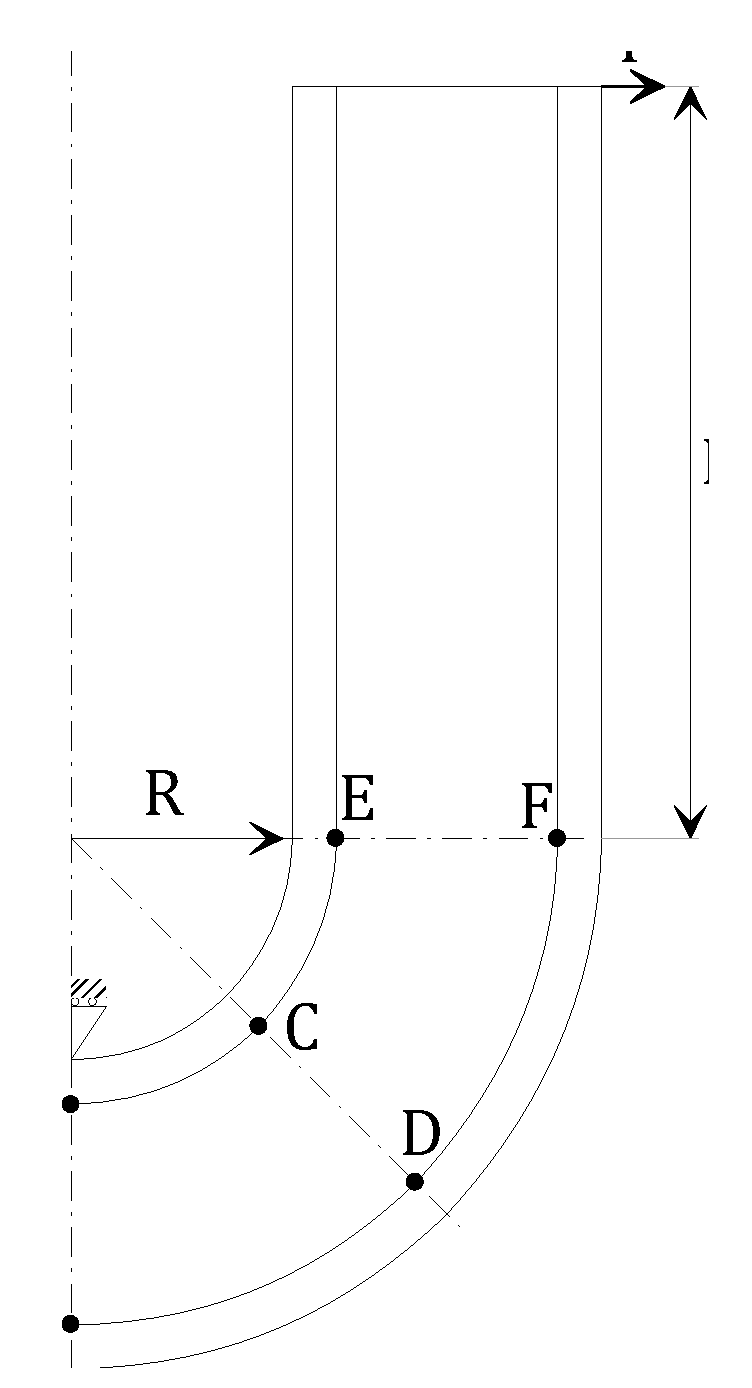
\includegraphics[height=80mm]{U-geo.eps} \hfill
  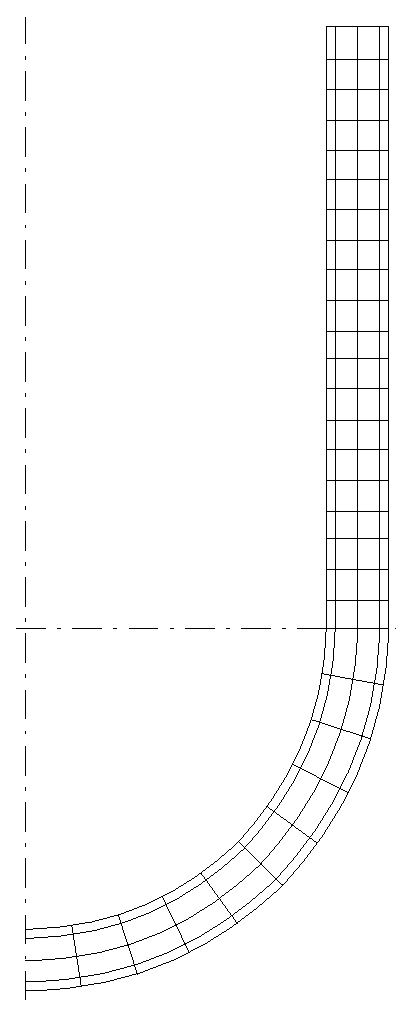
\includegraphics[height=80mm]{U-mesh1.eps}\hfill
  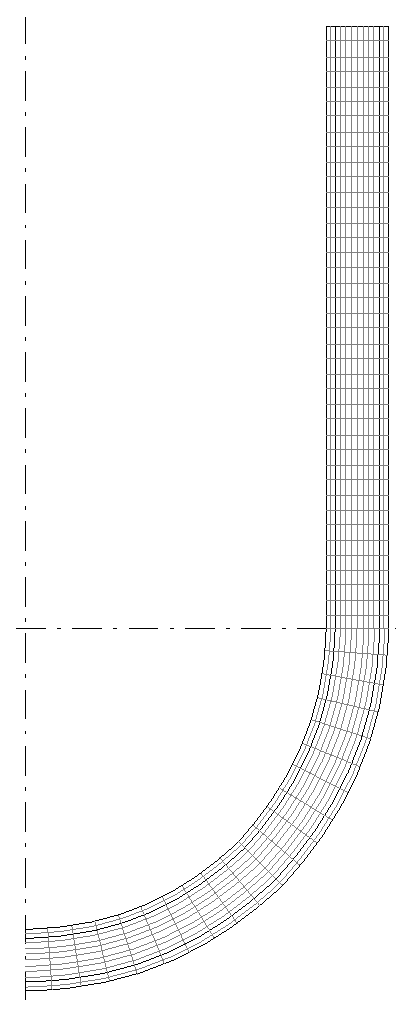
\includegraphics[height=80mm]{U-mesh2.eps}
  \caption{\label{Fig-poutU-geo} a) Géométrie de la poutre en U, b) le maillage utilisé pour le tester la méthode Reissner local, c) maillage permettant d'obtenir la «solution de référence» puisqu'il n'y a pas de solution analytique}
\end{figure}

Disposant de la macro précédente, nous allons l'appliquer au calcul de la poutre en~$U$ présentée à la figure~\ref{Fig-poutU-geo}a.
Il s'agit d'une poutre sandwich dont les peaux sont en aluminium et l'âme en résine époxy. Par symétrie, seule une demi-poutre est modélisée. Elle est soumise à une force unitaire sur chaque montant.
Les points pour lesquels nous nous intéresserons aux contraintes sont les points indiqués sur la \fig{Fig-poutU-geo}a, à savoir les points A, B, C, D, E et F.

\medskip
Le listing \ansys est le suivant:

\color{gris}\scriptsize
\begin{multicols}{2}
\begin{Verbatim}[numbers=left,numbersep=3pt]
!* geom: partie droite
long=20
H1=0.2
H2=1.8
H3=2
!*
!* geom coude
Rint=10
Rh1=Rint+H1
Rh2=Rint+H2
Rh3=Rint+H3
!*
!* maillage
NCUTS=40
NRCUTS=20
NCORE=16
NSKIN=2
Forc=1
!*
/PREP7
!*
ET,1,PLANE82
!*
UIMP,1,EX, , ,70000,
UIMP,1,NUXY, , ,0.3,
UIMP,1,EMIS, , ,1,
!*
!*
UIMP,2,EX, , ,3400,
UIMP,2,NUXY, , ,0.34,
UIMP,2,EMIS, , ,1,
!*
k,1,0,-Rh3
k,2,Rh3,0
k,3,Rh2,0
k,4,0,-Rh2
k,5,0,-Rh1
k,6,Rh1,0
k,7,Rint,0
k,8,0,-Rint
k,9,Rh3,long
k,10,Rh2,long
k,11,Rh1,long
k,12,Rint,long
k,13,0,0
!*
larc,1,2,13,Rh3,NRCUTS
l,2,3,NSKIN
larc,4,3,13,Rh2,NRCUTS
l,1,4,NSKIN
l,4,5,NCORE
l,3,6,NCORE
larc,5,6,13,Rh1,NRCUTS
l,5,8,NSKIN
larc,8,7,13,Rint,NRCUTS
l,6,7,NSKIN
!*
l,2,9,NCUTS
l,9,10,NSKIN
l,10,3,NCUTS
l,10,11,NCORE
l,11,6,NCUTS
l,11,12,NSKIN
l,12,7,NCUTS
!*
mat,1
a,1,2,3,4
a,5,6,7,8
a,2,9,10,3
a,6,11,12,7
mat,2
a,4,3,6,5
a,3,10,11,6
mat,1
amesh,1
amesh,2
amesh,3
amesh,4
mat,2
amesh,5
amesh,6
!*
DL,4,,symm
DL,5,,symm
DL,8,,symm
!*
dk,8,uy,0
!*
fk,9,fx,Forc
!*
FINISH
/SOLU
/STAT,SOLU
SOLVE
FINISH
/POST1
pldisp,1
*USE,INTERF
...
\end{Verbatim}
\end{multicols}
\color{black}\normalsize

On utilise la macro en tapant \verb|*USE,INTERF|, et les contraintes sont directement modifiées dans \ansys. On peut alors utiliser les mêmes fonctions qu'habituellement pour visualiser les différentes composantes des contraintes.


\medskip
Le listing Cast3M du même problème est le suivant:

\color{gris}\scriptsize
\begin{multicols}{2}
\begin{Verbatim}[numbers=left,numbersep=3pt]
* geom: partie droite
long=20.0;
H1=0.2;
H2=1.8;
H3=2.0;
*
* geom coude
Rint=10.0;
Rh1=Rint+H1;
Rh2=Rint+H2;
Rh3=Rint+H3;
MRint = -1. * Rint;
MRh1 = -1. * Rh1;
MRh2 = -1. * Rh2;
MRh3 = -1. * Rh3;
*
* maillage
NCUTS=40;
NRCUTS=20;
NCORE=16;
NSKIN=2;
Forc=1.0;
*
OPTION DIMENSION 2 ELEMENT QUA4;
*
k1 = 0. MRh3;
k2 = Rh3 0.;
k3 = Rh2 0.;
k4 = 0. MRh2;
k5 = 0. MRh1;
k6 = Rh1 0.;
k7 = Rint 0.;
k8 = 0. MRint;
k9 = Rh3 long;
k10 = Rh2 long;
k11 = Rh1 long;
k12 = Rint long;
k13 = 0. 0.;
*
L1 = CERCLE NRCUTS k1 k13 k2 ;
L2 = DROITE k2 k3 NSKIN;
L3 = CERCLE NRCUTS k4 k13 k3 ;
L4 = DROITE k1 k4 NSKIN;
L5 = DROITE k4 k5 NCORE;
L6 = DROITE k3 k6 NCORE;
L7 = CERCLE NRCUTS k5 k13 k6 ;
L8 = DROITE k5 k8 NSKIN;
L9 = CERCLE NRCUTS k8 k13 k7 ;
L10 = DROITE k6 k7 NSKIN;
*
L11 = DROITE k2 k9 NCUTS;
L12 = DROITE k9 k10 NSKIN;
L13 = DROITE k10 k3 NCUTS;
L14 = DROITE k10 k11 NCORE;
L15 = DROITE k11 k6 NCUTS;
L16 = DROITE k11 k12 NSKIN;
L17 = DROITE k12 k7 NCUTS;
*
SURF1 = DALLER L1 L2 L3 L4;
SURF2 = DALLER L2 L11 L12 L13;
PEAUEXT = SURF1 ET SURF2;
* ELIMINE PEAUEXT;
SURF1 = DALLER L3 L6 L7 L5;
SURF2 = DALLER L6 L13 L14 L15;
AME = SURF1 ET SURF2;
* ELIMINE AME;
SURF1 = DALLER L8 L7 L10 L9;
SURF2 = DALLER L10 L15 L16 L17;
PEAUINT = SURF1 ET SURF2;
* ELIMINE PEAUINT;
PoutU = PEAUEXT ET AME ET PEAUINT;
*
Model1 = MODL peauext MECANIQUE ELASTIQUE ISOTROPE QUA4;
Model2 = MODL ame MECANIQUE ELASTIQUE ISOTROPE QUA4;
Model3 = MODL peauint MECANIQUE ELASTIQUE ISOTROPE QUA4;
ModelTot = Model1 ET Model2 ET Model3;
*
Mater1=MATERIAU Model1 YOUNG 70000.0 NU 0.3 RHO 2700.0;
Mater2=MATERIAU Model2 YOUNG 3400.0 NU 0.34 RHO 1000.0;
Mater3=MATERIAU Model3 YOUNG 70000.0 NU 0.3 RHO 2700.0;
*
MR1 = RIGIDITE Model1 Mater1;
MR2 = RIGIDITE Model2 Mater2;
MR3 = RIGIDITE Model3 Mater3;
Mrigid = MR1 ET MR2 ET MR3;
*
CondL2 = BLOQUER UX (L4 ET L5 ET L8);
CondL1 = BLOQUER UY k8;
CondLtot = CondL1 ET CondL2;
FOR1 = FORCE(Forc 0.) k9;
Mrigid = Mrigid ET CondLtot;
*
Depl1 = RESOUD Mrigid For1 ;
*
UX1 = EXCO 'UX' depl1;
UY1 = EXCO 'UY' depl1;
Trace UX1 PoutU;
Trace UY1 PoutU;
*
def0 = DEFORMEE poutU Depl1 0.0 BLEU;
def1 = DEFORMEE poutU Depl1 ROUGE;
trace (def0 ET def1);
* ...
\end{Verbatim}
\end{multicols}
\color{black}\normalsize
Il reste maintenant à avoir les résultats dans les repères locaux élémentaires,
et voir ce qui se passe aux interfaces...




\medskip
\subsection{Résultats}

Dans les listings ci-dessus, nous n'avons pas exposé comme atteindre les contraintes, car cela sera fait en TP.
Les résultats directement obtenus sont donnés à la \fig{Fig-poutU-disp} pour la déformée et les déplacements selon~$x$ et~$y$, et à la \fig{Fig-poutU-eps} pour les déformations.
\begin{figure}[h!]
  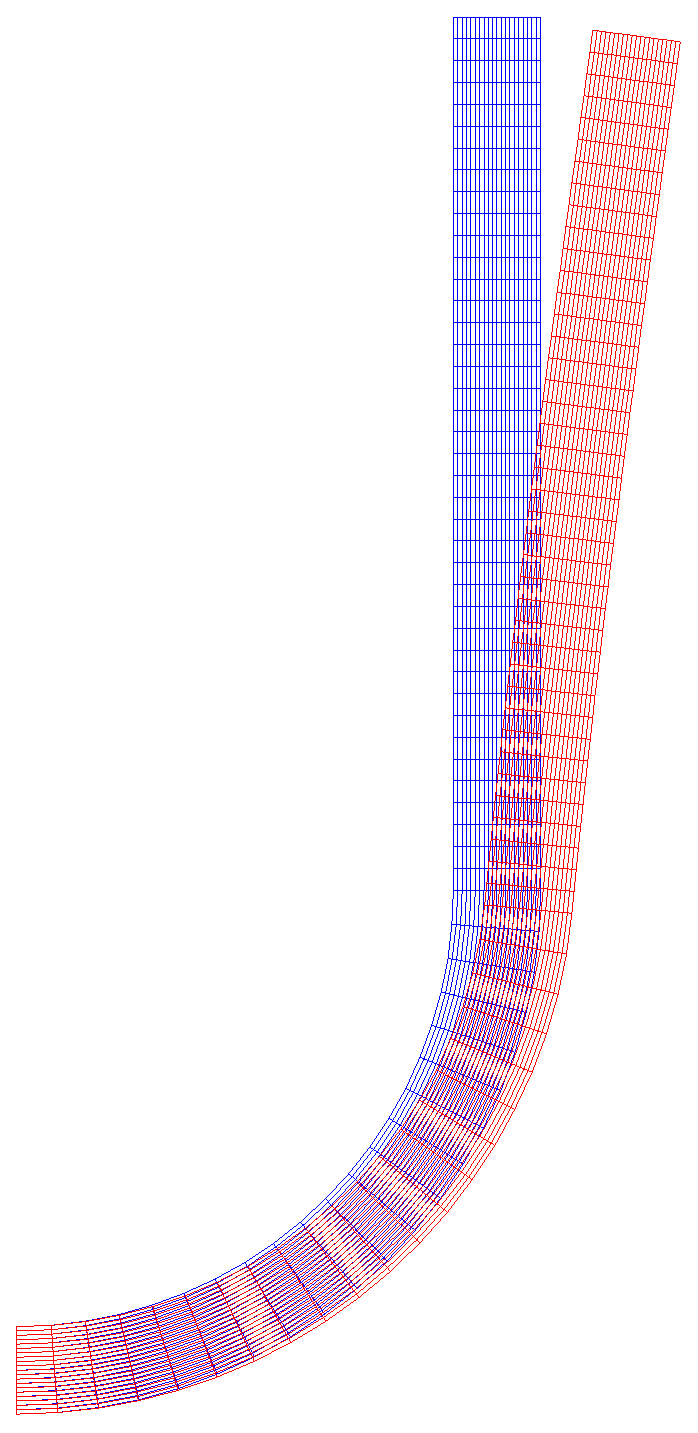
\includegraphics[height=80mm]{U-def.eps} \hfill
  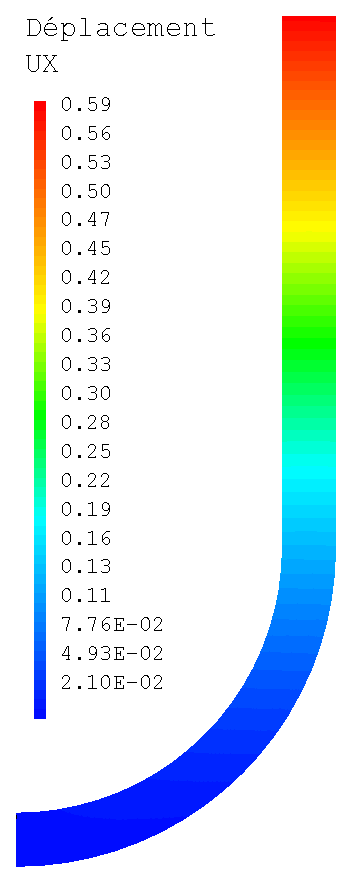
\includegraphics[height=80mm]{U-ux.eps}\hfill
  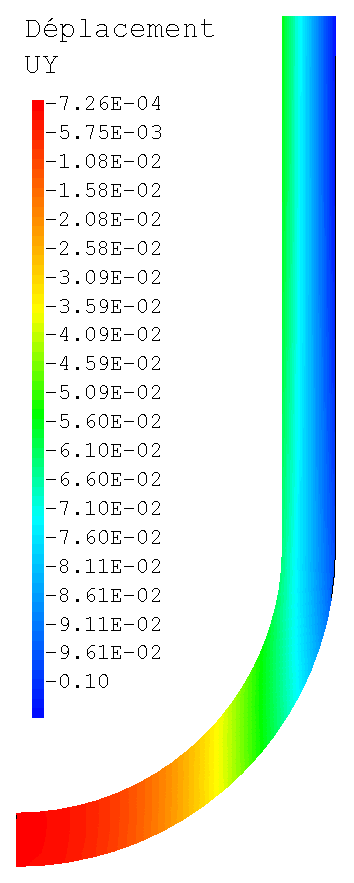
\includegraphics[height=80mm]{U-uy.eps}
  \caption{\label{Fig-poutU-disp} Déformée et déplacements}
\end{figure}
\begin{figure}[h!]
  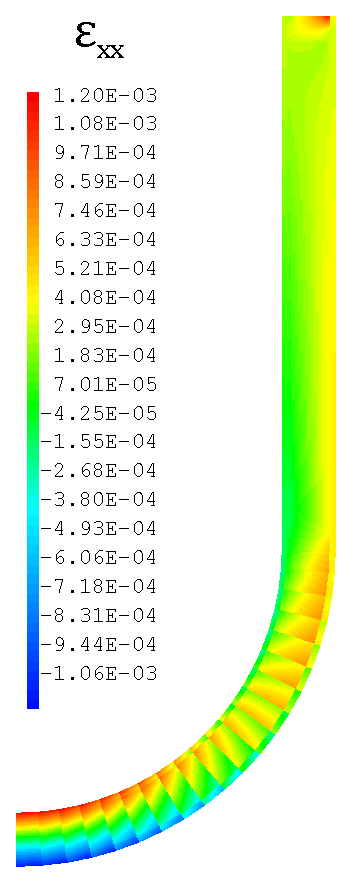
\includegraphics[height=80mm]{U-epsXX.eps} \hfill
  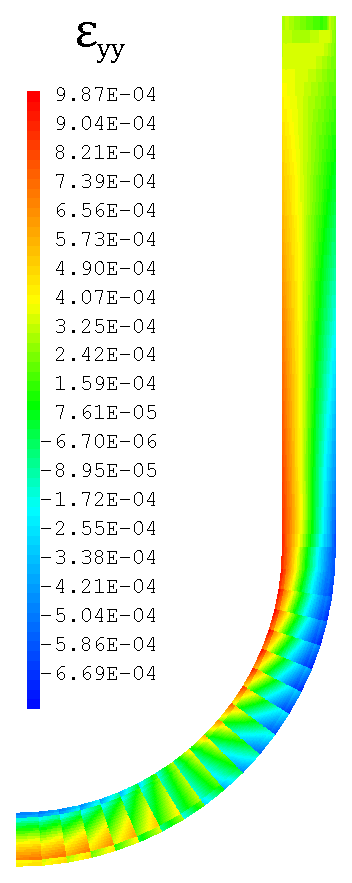
\includegraphics[height=80mm]{U-epsYY.eps}\hfill
  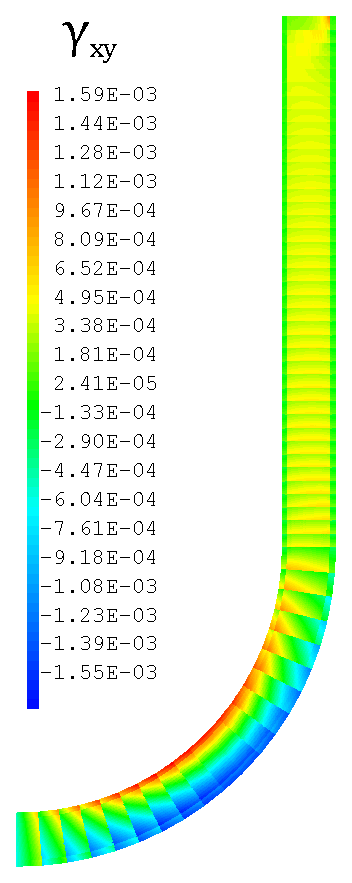
\includegraphics[height=80mm]{U-epsXY.eps}
  \caption{\label{Fig-poutU-eps} Déformations}\label{VMtiti}
\end{figure}

\medskip
Néanmoins nous présentons quelques résultats issus de l'analyse des contraintes aux interfaces avec ou sans utilisation de la méthode de Reissner local. Nous nous concentrerons sur les résultats numériques et graphiques permettant d'apprécier la précision de la méthode de Reissner local par rapport aux résultats d'\ansys aux points~$A$, $B$, $E$ et~$F$ ainsi que d'étudier l'influence de la valeur du rayon~$R$.

\medskip
Une première remarque s'impose: plus la valeur du rayon est faible, plus les résultats sont mauvais, quelle que soit la méthode employée (et vous devez savoir pourquoi à ce niveau du document).

\medskip
Au point~$A$, l'influence des conditions aux limites est encore sensible: en plus de la condition de symétrie de la structure, le blocage du déplacement vertical induit une légère détérioration des résultats numériques. L'influence de cette condition aux limites n'est plus visible au point~$B$.

\medskip
En~$A$ et~$B$, la composante discontinue est~$\sigma_{xx}$, les composantes~$\sigma_{yy}$ et~$\sigma_{xy}$ sont continues. Par contre, aux points~$E$ et~$F$, c'est~$\sigma_{yy}$ la composante discontinue et~$\sigma_{xx}$ et $\sigma_{xy}$ les composantes continues.

\medskip
D'après les résultats présentés ci-après, il est visible que la méthode de Reissner local permet d'améliorer les résultats par rapport à \ansys.



\begin{table}[h!]\label{VMtoto}
\centering\small
  \begin{tabular}{|l||r|r|r|r|r|}
   \hline
   \multicolumn{1}{|c||}{\raisebox{-2.5mm}{Méthode}}&
   \multicolumn{1}{c}{\raisebox{-2.5mm}{$R$}}&
   \multicolumn{1}{|c}{$\sigma_{xx}$}&
   \multicolumn{1}{|c}{$\sigma_{xx}$}&
   \multicolumn{1}{|c}{\raisebox{-2.5mm}{$\sigma_{yy}$}}&
   \multicolumn{1}{|c|}{\raisebox{-2.5mm}{$\sigma_{xy}$}}\\[-3mm]
   &&
   \multicolumn{1}{|c}{peau}&
   \multicolumn{1}{|c|}{âme}&&\\
   &(mm)&
   \multicolumn{1}{|c}{(MPa)}&
   \multicolumn{1}{|c|}{(MPa)}&
   \multicolumn{1}{|c|}{(MPa)}&
   \multicolumn{1}{|c|}{(MPa)}\\
   \hline
   \hline
   Ref &10 &72,085 &4,0121 &1,5883 &-0,0023339  \\
   Reiss&10 &71,957 &3,9670 &1,5987 &-0,0155720  \\
   \ansys&10&71,957 &3,9670 & 1,5116 & 0,0086231  \\
   \hline
   Ref &8 &66,500 &3,8400 &1,8556 &-0,0022273  \\
   Reiss&8 &66,665 &3,7863 &1,8888 &-0,0118667  \\
   \ansys&8 &66,665 &3,7863 & 1,7943 & 0,0111910  \\
   \hline
   Ref &5 &57,289 &3,6598 &2,6317 &-0,0018770  \\
   Reiss&5 &57,727 &3,5771 &2,6979 &-0,0071024  \\
   \ansys&5 &57,727 &3,5771 & 2,6066 & 0,0128210  \\
   \hline
   Ref &3 &49,551 &3,6827 &3,9304 &-0,0014368  \\
   Reiss&3 &49,454 &3,5552 &4,0110 &-0,0046055  \\
   \ansys&3 &49,454 &3,5552 & 3,9621 & 0,0106410  \\
   \hline
   Ref &2 &42,699 &3,8289 &5,4227 &-0,0009727  \\
   Reiss&2 &42,362 &3,6593 &5,4785 &-0,0037443  \\
   \ansys&2 &42,362 &3,6593 & 5,5264 & 0,0059470  \\
   \hline
   Ref &1 &27,171 &4,3142 &9,2850 &-0,0004173  \\
   Reiss&1 &25,876 &4,0707 &9,1122 &-0,0021565  \\
   \ansys&1 &25,876 &4,0707 &9,6345 & 0,0005231  \\
   \hline
  \end{tabular}
\caption{\label{Tab:pt-A} Résultats au point~$A$}
\end{table}

%\begin{figure}
%\centering
%\input{tex/a-sxxc.2012.txt}
%
%  \caption{\label{Fig:asxxc}~$\sigma_{xx}$ dans l'âme en~$A$}
%\end{figure}
%
%\begin{figure}
%\centering
%\input{tex/a-sxxs.2012.txt}
%
%  \caption{\label{Fig:asxxs}~$\sigma_{xx}$ dans la peau en~$A$}
%\end{figure}

\ifVMSurLaMemePage\clearpage\fi
\begin{figure}[h!]
\centering
\input{tex/a-syy.2012.txt}
\caption{\label{Fig:asyy}~$\sigma_{yy}$ en~$A$}
\end{figure}

\ifVMSurLaMemePage\else\clearpage\fi
\begin{figure}[h!]
\centering
\input{tex/a-sxy.2012.txt}
\caption{\label{Fig:asxy}~$\sigma_{xy}$ en~$A$}
\end{figure}

\ifVMSurLaMemePage\clearpage\fi
\begin{table}[h!]
\centering\small
  \begin{tabular}{|l||r|c|c|c|c|}
   \hline
   \multicolumn{1}{|c||}{\raisebox{-2.5mm}{Méthode}}&
   \multicolumn{1}{c}{\raisebox{-2.5mm}{$R$}}&
   \multicolumn{1}{|c}{$\sigma_{xx}$}&
   \multicolumn{1}{|c}{$\sigma_{xx}$}&
   \multicolumn{1}{|c}{\raisebox{-2.5mm}{$\sigma_{yy}$}}&
   \multicolumn{1}{|c|}{\raisebox{-2.5mm}{$\sigma_{xy}$}}\\[-3mm]
   &&
   \multicolumn{1}{|c}{peau}&
   \multicolumn{1}{|c|}{âme}&&\\
   &(mm)&
   \multicolumn{1}{|c}{(MPa)}&
   \multicolumn{1}{|c|}{(MPa)}&
   \multicolumn{1}{|c|}{(MPa)}&
   \multicolumn{1}{|c|}{(MPa)}\\
   \hline
   \hline
   Ref& 10 & -72,248 & -3,0668 & 1,4080 & -0,0023570 \\
   Reiss&10 & -72,542 & -3,1193 & 1,2573 & -0,0138800 \\
   \ansys&10& -72,542 & -3,1193 & 1,5464 & -0,0198700 \\
   \hline
   Ref& 8 & -67,723 & -2,7905 & 1,5799 & -0,0026011 \\
   Reiss&8 & -68,001 & -2,8457 & 1,4570 & -0,0107700 \\
   \ansys&8 & -68,001 & -2,8457 & 1,7111 & -0,0197300 \\
   \hline
   Ref& 5 & -61,079 & -2,3199 & 2,0320 & -0,0024099 \\
   Reiss&5 & -61,335 & -2,3813 & 1,9460 & -0,0067001 \\
   \ansys&5 & -61,335 & -2,3813 & 2,1535 & -0,0186210 \\
   \hline
   Ref& 3 & -56,823 & -1,9080 & 2,6611 & -0,0022154 \\
   Reiss&3 & -57,072 & -1,9756 & 2,5888 & -0,0045050 \\
   \ansys&3 & -57,072 & -1,9756 & 2,7738 & -0,0176540 \\
   \hline
   Ref& 2 & -54,772 & -1,6200 & 3,2396 & -0,0021234 \\
   Reiss&2 & -55,026 & -1,6902 & 3,1612 & -0,0036124 \\
   \ansys&2 & -55,026 & -1,6902 & 3,3438 & -0,0172760 \\
   \hline
   Ref& 1 & -52,491 & -1,1687 & 4,2871 & -0,0020797 \\
   Reiss&1 & -52,777 & -1,2391 & 4,1625 & -0,0031088 \\
   \ansys&1 & -52,777 & -1,2391 & 4,3710 & -0,0174200 \\
   \hline
  \end{tabular}
  \caption{\label{Tab:pt-B} Résultats au point~$B$}
\end{table}
%\clearpage
%\begin{figure}
%\centering
%\input{tex/b-sxxc.2012.txt}
%
%  \caption{\label{Fig:bsxxc}~$\sigma_{xx}$ dans l'âme en~$B$}
%\end{figure}
%
%\begin{figure}
%\centering
%\input{tex/b-sxxs.2012.txt}
%
%  \caption{\label{Fig:bsxxs}~$\sigma_{xx}$ dans la peau en~$B$}
%\end{figure}
%

\ifVMSurLaMemePage\else\clearpage\fi
\begin{figure}[h!]
\centering
\input{tex/b-syy.2012.txt}
\caption{\label{Fig:bsyy}~$\sigma_{yy}$ en~$B$}
\end{figure}

\ifVMSurLaMemePage\clearpage\fi
\begin{figure}[h!]
\centering
\input{tex/b-sxy.2012.txt}
\caption{\label{Fig:bsxy}~$\sigma_{xy}$ en~$B$}
\end{figure}

\ifVMSurLaMemePage\else\clearpage\fi
\begin{table}[h!]
\centering\small
  \begin{tabular}{|l||r|c|c|c|c|}
   \hline
   \multicolumn{1}{|c||}{\raisebox{-2.5mm}{Méthode}}&
   \multicolumn{1}{c}{\raisebox{-2.5mm}{$R$}}&
   \multicolumn{1}{|c}{$\sigma_{yy}$}&
   \multicolumn{1}{|c}{$\sigma_{yy}$}&
   \multicolumn{1}{|c}{\raisebox{-2.5mm}{$\sigma_{xx}$}}&
   \multicolumn{1}{|c|}{\raisebox{-2.5mm}{$\sigma_{xy}$}}\\[-3mm]
   &&
   \multicolumn{1}{|c}{peau}&
   \multicolumn{1}{|c|}{âme}&&\\
   &(mm)&
   \multicolumn{1}{|c}{(MPa)}&
   \multicolumn{1}{|c|}{(MPa)}&
   \multicolumn{1}{|c|}{(MPa)}&
   \multicolumn{1}{|c|}{(MPa)}\\
   \hline
   \hline
   ref& 10 &46,0340 &2,410200 &0,57548 &0,77518 \\
   Reiss&10 &46,0265 &2,397450 &0,48986 &0,71342 \\
   \ansys&10&46,0265 &2,397450 &0,62529 &0,80572 \\
   \hline
   ref& 8  &45,8625 &2,443000 &0,68465 &0,83563 \\
   Reiss&8 &45,8505 &2,421450 &0,62992 &0,76781 \\
   \ansys&8 &45,8505 &2,421450 &0,71910 &0,90760 \\
   \hline
   ref& 5  &45,4490 &2,539450 &1,00620 &1,00390 \\
   Reiss&5 &45,5025 &2,499550 &1,00810 &0,91559 \\
   \ansys&5 &45,5025 &2,499550 &0,94099 &1,19800 \\
   \hline
   ref& 3  &44,5760 &2,694400 &1,56820 &1,25790 \\
   Reiss&3 &45,0015 &2,644550 &1,62260 &1,10690 \\
   \ansys&3 &45,0015 &2,644550 &1,30760 &1,64980 \\
   \hline
   ref& 2  &43,1510 &2,856600 &2,23920 &1,50420 \\
   Reiss&2 &44,1375 &2,805000 &2,32600 &1,25870 \\
   \ansys&2 &44,1375 &2,805000 &1,77080 &2,12250 \\
   \hline
   ref& 1  &37,6330 &3,184100 &4,02110 &1,90380 \\
   Reiss&1 &40,1735 &3,143850 &4,04390 &1,41220 \\
   \ansys&1 &40,1735 &3,143850 &3,04360 &3,15350 \\
   \hline
  \end{tabular}
  \caption{\label{Tab:pt-E} Résultats au point~$E$}
\end{table}

%\begin{figure}
%\centering
%\input{tex/e-sxxc.2012.txt}
%
%  \caption{\label{Fig:esxxc}~$\sigma_{yy}$ dans l'âme en~$E$}
%\end{figure}
%
%\begin{figure}
%\centering
%\input{tex/e-sxxs.2012.txt}
%
%  \caption{\label{Fig:esxxs}~$\sigma_{yy}$ dans la peau en~$E$}
%\end{figure}
%

\ifVMSurLaMemePage\clearpage\fi
\begin{figure}[h!]
\centering
\input{tex/e-syy.2012.txt}
\caption{\label{Fig:esyy}~$\sigma_{xx}$ en~$E$}
\end{figure}

\ifVMSurLaMemePage\else\clearpage\fi
\begin{figure}[h!]
\centering
\input{tex/e-sxy.2012.txt}
\caption{\label{Fig:esxy}~$\sigma_{xy}$ en~$E$}
\end{figure}

\ifVMSurLaMemePage\clearpage\fi
\begin{table}[h!]
\centering\small
  \begin{tabular}{|l||r|c|c|c|c|}
   \hline
   \multicolumn{1}{|c||}{\raisebox{-2.5mm}{Méthode}}&
   \multicolumn{1}{c}{\raisebox{-2.5mm}{$R$}}&
   \multicolumn{1}{|c}{$\sigma_{yy}$}&
   \multicolumn{1}{|c}{$\sigma_{yy}$}&
   \multicolumn{1}{|c}{\raisebox{-2.5mm}{$\sigma_{xx}$}}&
   \multicolumn{1}{|c|}{\raisebox{-2.5mm}{$\sigma_{xy}$}}\\[-3mm]
   &&
   \multicolumn{1}{|c}{peau}&
   \multicolumn{1}{|c|}{âme}&&\\
   &(mm)&
   \multicolumn{1}{|c}{(MPa)}&
   \multicolumn{1}{|c|}{(MPa)}&
   \multicolumn{1}{|c|}{(MPa)}&
   \multicolumn{1}{|c|}{(MPa)}\\
   \hline
   \hline
   ref & 10 & -47,438 &-2,1425 &0,54431 & 0,30073 \\
   Reiss&10 & -47,510 &-2,1533 &0,39416 & 0.38936 \\
   \ansys&10& -47,510 &-2,1533 &0,65814 & 0,30000 \\
   \hline
   ref & 8 & -47,4555 &-2,11415 &0,62480 & 0,24743 \\
   Reiss&8 & -47,5605 &-2,12825 &0,50447 & 0.33138 \\
   \ansys&8 & -47,5605 &-2,12825 &0,72921 & 0,21663 \\
   \hline
   ref & 5 & -47,415 &-2,03645 &0,83167 & 0,10558 \\
   Reiss&5 & -47,5335 &-2,05940 &0,76054 & 0,18360 \\
   \ansys&5 & -47,5335 &-2,05940 &0,87666 & 0,00251 \\
   \hline
   ref & 3 & -47,223 &-1,92305 &1,11940 &-0,10042 \\
   Reiss&3 & -47,1885 &-1,95170 &1,07760 &-0,01314 \\
   \ansys&3 & -47,1885 &-1,95170 &1,05090 &-0,28747 \\
   \hline
   ref & 2 & -46,940 &-1,81445 &1,38480 &-0,29901 \\
   Reiss&2 & -46,6760 &-1,84130 &1,35230 &-0,18934 \\
   \ansys&2 & -46,6760 &-1,84130 &1,21420 &-0,55238 \\
   \hline
   ref & 1 & -46,1935 &-1,61030 &1,85860 &-0,67358 \\
   Reiss&1 & -45,4620 &-1,62185 &1,81270 &-0,50497 \\
   \ansys&1 & -45,4620 &-1,62185 &1,52280 &-1,03400 \\
   \hline
  \end{tabular}
\caption{\label{Tab:pt-F} Résultats au point~$F$}
\end{table}

%\begin{figure}
%\centering
%\input{tex/f-sxxc.2012.txt}
%
%  \caption{\label{Fig:fsxxc}~$\sigma_{yy}$ dans l'âme en~$F$}
%\end{figure}
%
%\clearpage
%
%\begin{figure}
%\centering
%\input{tex/f-sxxs.2012.txt}
%
%  \caption{\label{Fig:fsxxs}~$\sigma_{yy}$ dans la peau en~$F$}
%\end{figure}

\ifVMSurLaMemePage\else\clearpage\fi
\begin{figure}[h!]
\centering
\input{tex/f-syy.2012.txt}
\caption{\label{Fig:fsyy}~$\sigma_{xx}$ en~$F$}
\end{figure}

\ifVMSurLaMemePage\clearpage\fi
\begin{figure}[h!]
\centering
\input{tex/f-sxy.2012.txt}
\caption{\label{Fig:fsxy}~$\sigma_{xy}$ en~$F$}
\end{figure}
%\clearpage
